
\titleformat{\chapter}[display]{\normalfont\LARGE\bfseries}{}{1em}{\thechapter.~}

\chapter{Laboratorio:  Arranques a tensión reducida y circuitos temporizados.}

\section{Objetivos}
Este  laboratorio busca:
\begin{itemize}
	{\small
	 \item Diseñar un circuito secuencial temporizado que permita arrancar un motor en tensión reducida utilizando el método de estrella delta.
    \item  Diseñar un circuito secuencial temporizado que permita arrancar un motor mediante auto-transformador.
    \item  Diseñar un circuito secuencial temporizado que permita arrancar en cascada dos motores y apagarlos en cascada. 
	 \item Alambrar el circuito de control y potencia.
	 \item Detectar fallas en circuitos alambrados con lógica cableada.
	 
 }
\end{itemize} 

 
\section{Equipos y materiales}
Para este laboratorio de necesitaran:
\begin{itemize}
	{\small \item 2 motor trifásico 1/2 hp de 3 puntas.
	\item 1 motor trifásico 1/2 hp de 6 puntas.
	\item 2 relevadores térmico.
	\item 4 contactores.
	\item 1 botón pulsar cerrado.
	\item 2 botones pulsadores abiertos.
	\item 1 temporizador On-Delay.
	\item 1 temporizador Off-Delay.
	\item 1 amperimetro de gancho con medición INRUSH.
	\item 1 Analizador de señales Fluke 143B
}
\end{itemize}

\section{Marco de referencia}
El arranque de motores trifásicos a tensión reducida es una técnica utilizada para reducir la corriente de arranque y el par de arranque, lo que ayuda a evitar problemas de sobrecarga en el sistema eléctrico.

Existen diferentes técnicas, pero las más comunes son: de arranque a tensión reducida, como el arranque estrella-triángulo, el arranque con autotransformador, arranque con resistencias estatóricas o rotóricas, arrancadores suaves, etc. Cada técnica tiene sus propias ventajas y desventajas y debe seleccionarse en función de las características del motor, la aplicación y las limitaciones del sistema eléctrico.

\subsection{Temporizadores Electrónicos}

Los temporizadores son dispositivos de control de tiempo que permiten activar o desactivar algún actuador un tiempo después de activarse o desactivarse una señal de control. Los temperorizadores pueden ser  construidos de forma mecánica, neumática, electromecánica, electrónica, programada pero todos tienen funcionamientos estandarizados como: retardo a la conexión (On-delay), retardo a la desconexión (Off-delay), retardo a la conexión y desconexión (On/Off-Delay), relés de pulsos simétricos, entre otros. 

La Figura \ref{fig:imagen} muestra un temporizador electrónico y la Figura \ref{fig:Diagrama} su diagrama de conexión. Note que el dispositivo se alimenta mediante las borneras A1-A2,  las señales de control se declaran como X1 y Y1, y los contactos auxiliares normalmente cerrados y abiertos son las borneras 15-16-18 y 21-22-24. Este temporizador posee cuatro potenciometros o diales: el  primer dial selecciona el rango de tiempo $R$, con el segundo dial se selecciona un valor $V$ entre 1 y 10, el tiempo de activacion  $T$ se calcula como  $T=R\cdot V/10$. El tercer dial selecciona una de las ocho funciones preestablecidas: a modo de ejemplo la Figura \ref{fig:Funciones} muestra las funciones A, C, Ac que representan temporizador operando como: On-delay, Off-delay y On-Off delay. Finalmente el cuarto dial, permite establecer un tiempo de retardo entre los contactos auxiliares R1 y R2, más información se detalla en \cite{Scheneider4}.


\begin{figure}
	\centering
	\begin{subfigure}[b]{0.3\textwidth}
		\centering
		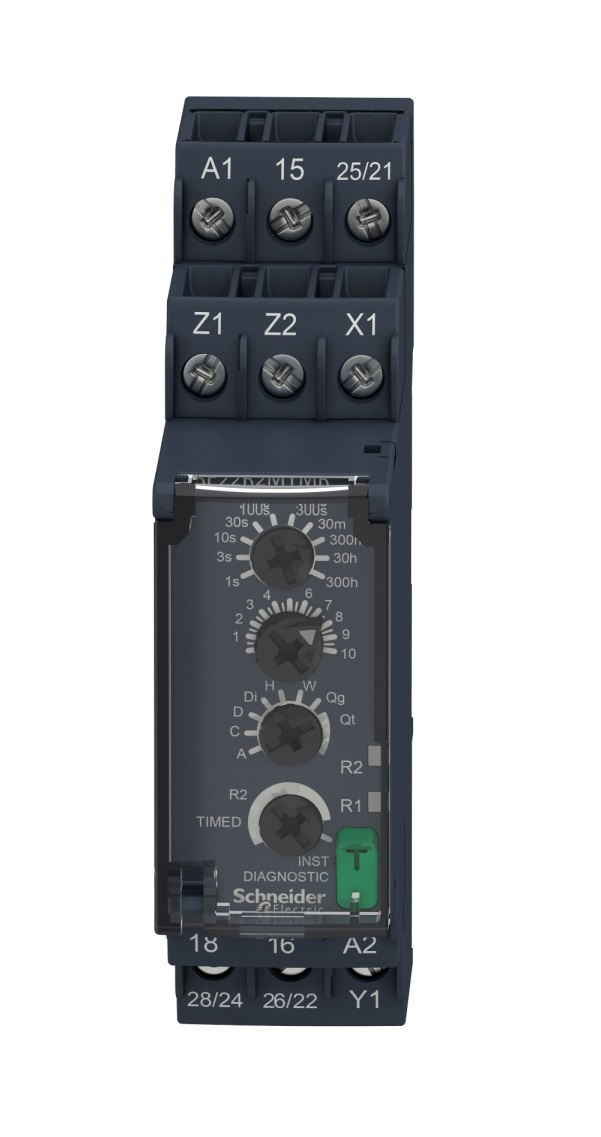
\includegraphics[width=\textwidth]{Imagenes/RE22R2MYMR}
		\caption{Temporizador RE22R2MYMR \cite{Scheneider3} }
		\label{fig:imagen}
	\end{subfigure}
	\hfill
	\begin{subfigure}[b]{0.5\textwidth}
		\centering
		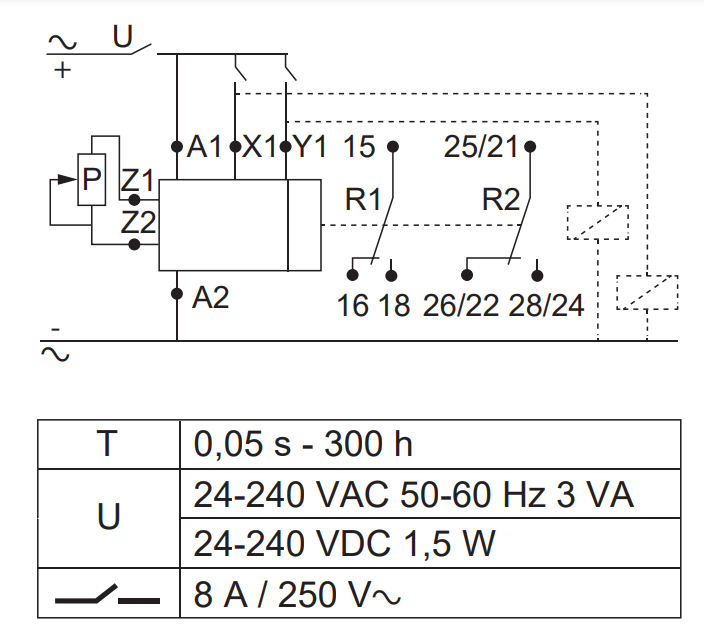
\includegraphics[width=\textwidth]{Imagenes/TimerDiagram}
		\caption{Diagrama de conexión del RE22R2MYMR \cite{Scheneider4} }
		\label{fig:Diagrama}
	\end{subfigure}
	\caption{Temporizador de 8 funciones RE22R2MYMR.}
\end{figure}



\begin{figure}
	\centering
	\begin{subfigure}[b]{0.32\textwidth}
		\centering
		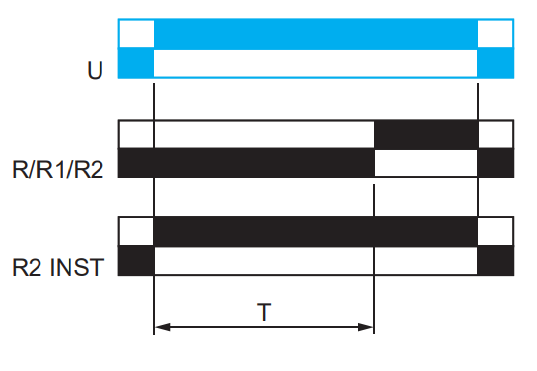
\includegraphics[width=\textwidth]{Imagenes/A-OnDelay}
		\caption{A: On delay }
		\label{fig:on-delay}
	\end{subfigure}
	\begin{subfigure}[b]{0.32\textwidth}
		\centering
		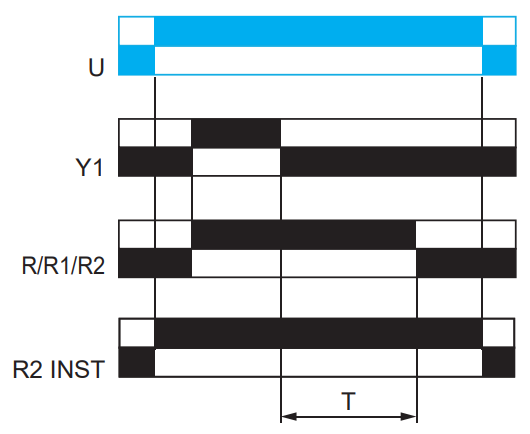
\includegraphics[width=\textwidth]{Imagenes/C-OffDelay}
		\caption{C: Off delay}
		\label{fig:Off-delay}
	\end{subfigure}
	\begin{subfigure}[b]{0.32\textwidth}
	\centering
	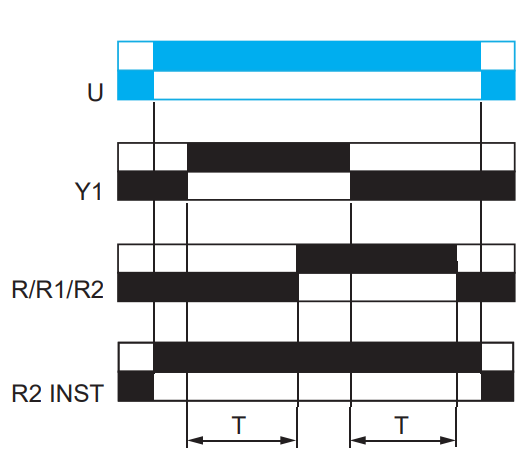
\includegraphics[width=\textwidth]{Imagenes/Ac-On-OffDelay}
	\caption{Ac: On-Off delay }
	\label{fig:OnOff-delay}
	\end{subfigure}
	\caption{Diagramas de tiempo de funciones a escoger en el selector del temporizador \cite{Scheneider4}.}
	\label{fig:Funciones}
\end{figure}



\subsection{Arranque a tensión reducida}

Los arranques a tensión reducida buscan reducir el voltaje que alimenta los devanados estatóricos para que en el momento del arranque la corriente de línea se reduzca.

El arranque por autotranformador, utilizado en motores trifásicos de inducción jaula de árdilla de tres terminales, permite reducir tanto el voltaje de línea como la corriente de linea que consume el motor. Si la relacion de tranformacion es $a=V_{out}/V_{in}$, donde $V_{out}$ es el voltaje hacia el motor y $V_{in}$ es el voltage de la red. La corriente de línea antes del autotransformador es $I_{linea} = a^{2}\cdot I_{arr}$, donde $I_{arr}$ es la corriente de arranque a tensión plena. La Figura \ref{fig:control-auto-transformador} muestra el circuito de potencia y control para el arranque por auto-transformador.

\begin{figure}
	\centering
	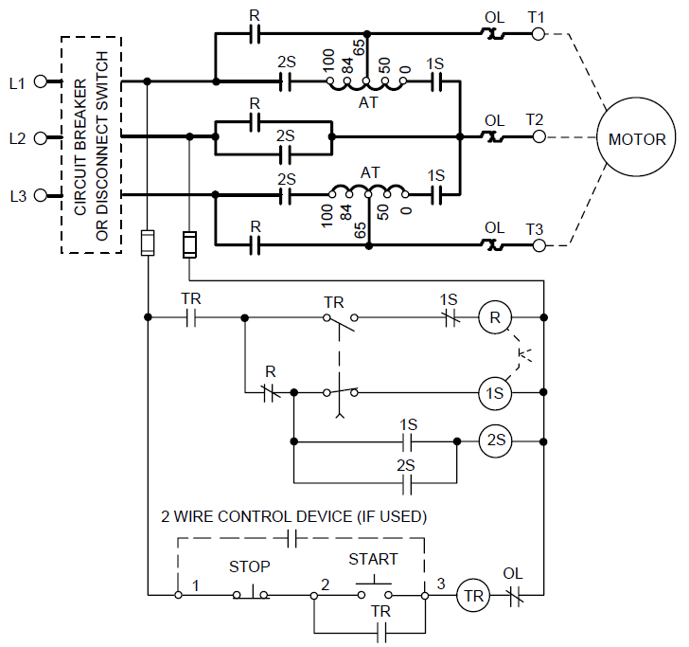
\includegraphics[width=0.6\linewidth]{Imagenes/Control-Auto-transformador}
	\caption{Arranque por auto-transformador con transición abierta \cite{Scheneider5}. }
	\label{fig:control-auto-transformador}
\end{figure}

Los motores trifásicos de indución jaula de ardilla de seis puntas se pueden arrancar realizando una reconfiguración de su devanado. Durante el régimen transitorio  sus devanados se alambran en estrella ($\leftthreetimes$) y cuando su velocidad alcanza el 80\% aproximadamente se realiza la re-conexión en delta ( $\Delta$) de los devanados. Esto permiten reducir el voltaje en $\sqrt{3}$ y la corriente de arranque se reduce a un tercio de la original. La Figura \ref{fig:potencia-estrella-delta} muestra el circuito de potencia para el arranque $\leftthreetimes-\Delta$.

\begin{figure}
	\begin{subfigure}[b]{0.49\textwidth}
		\centering
		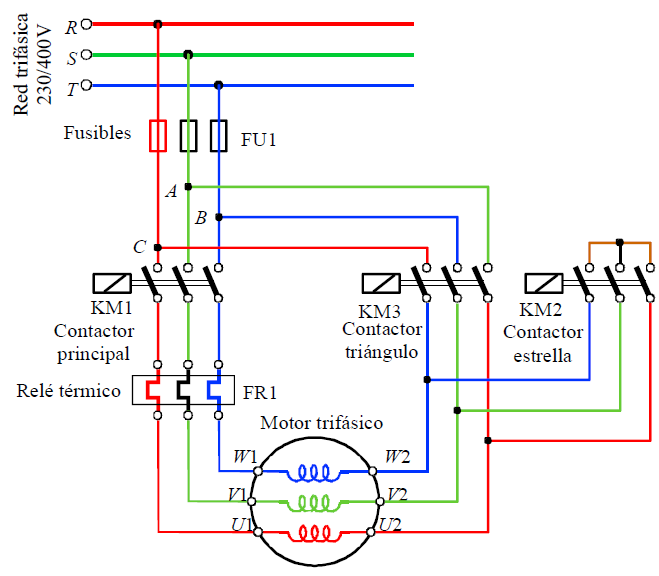
\includegraphics[width=\textwidth]{Imagenes/Potencia-Estrella-Delta}
		\caption{Circuito de potencia}
		\label{fig:potencia-estrella-delta}
	\end{subfigure}
	\begin{subfigure}[b]{0.49\textwidth}
		\centering
		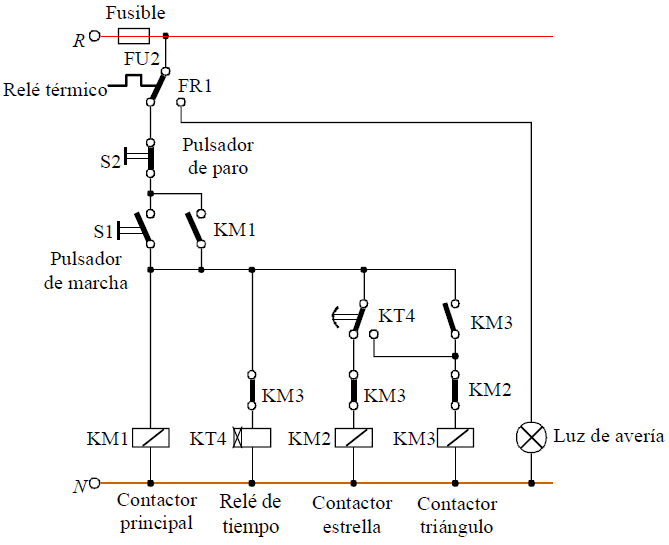
\includegraphics[width=\textwidth]{Imagenes/Control-Estrellla-Delta}
		\caption{Circuito de control}
		\label{fig:control-estrella-delta}
	\end{subfigure}
	\caption{Arranque Estrella-Delta transición abierta  \cite{Mora08}.}
\end{figure}



\section{Metodología}

Este laboratorio tiene una duración de 4 lecciones, repartidas en dos semanas. Los estudiantes deben mostrar durante las clases programadas las tres actividades propuestas. Deben recabar fotografías y resultados de los equipos de medición para elaborar las evidencias. Las evidencias se subirán al TecDigital la semana siguiente finalizadas las actividades.

\section{Práctica en Clase}

\subsection{Actividad 1}

El circuito de control y potencia del un arranque y pare secuencial de dos motores trifásicos de tres punta posee dos variantes.  La primera consiste en que cuando se presiona el botón de inicio, arranca el motor uno y un tiempo después el motor 2. Posteriormente cuando se presiona el botón de paro, el motor 1 se para y un tiempo después el motor 2.La segunda variantes consiste en el paro de los motores, cuando se presiona el botón de paro, el motor 2 se detiene y un tiempo después el motor 1.  

Si su carné termina en número impar, implemente la variante 1, si su carné terminar en número par implemente la variante 2.
 
\subsubsection{Conteste las preguntas}

¿Puede mostrar el circuito de control para ambas variantes y las ecuaciones lógicas?
¿Puede mostrar el diagrama de tiempos (oscilograma) del funcionamiento de cada bobina, y su relación con los eventos?
¿El circuito implementado funciona según lo planeado? ¿Cuanto es la corriente de arranque medida con el FLUKE 143B?

\subsection{Actividad 2}
 
 Realice un arranque por auto-transformador para un motor trifásico de tres puntas. Mida la corriente de arranque  y la tensión de alimentación del motor.
 
 
\subsubsection{Conteste las preguntas:}

¿Cual es la corriente de arranque del motor según su dato de placa y letra de código? ¿Cuanto es la corriente de arranque medida con el FLUKE 143B? ¿Cuanto se redujo la corriente en el arranque?¿Se cumple la ecuación $I_{linea} = a^{2}\cdot I_{arr}$ ?

\subsection{Actividad 3}

Realice un arranque pare reversible para un motor que arranca en estrella-delta. Es decir, el motor debe arrancar en estrella-delta hacia la derecha, o puede arrancar en estrella-delta hacia la izquierda. Cuando se presiona el botón de pare o sobrecarga este se detiene. Solo se requiere un temporizador tipo On-Delay.

\subsubsection{Conteste las preguntas:} 

 ¿Como es el circuito implementado? ¿Cuanto es la corriente de arranque medida con el FLUKE 143B? ¿Como es el diagrama de tiempos de cada bobina? ¿La corriente de arranque se redujo un tercio del arranque a plena tensión? 



